\chapter{Garment Depth Map Clustering}
\label{garment_clustering}

This chapter explains in detail the Garment Depth Map Clustering stage that our algorithm performs to the garment data previously segmented to group similar height regions of the garment. Some of these clusters represent overlapped regions of the garment. The block diagram of this stage can be seen in Figure \ref{fig:garment_clustering_blocks}.

\begin{figure}[thpb]
    \centering
    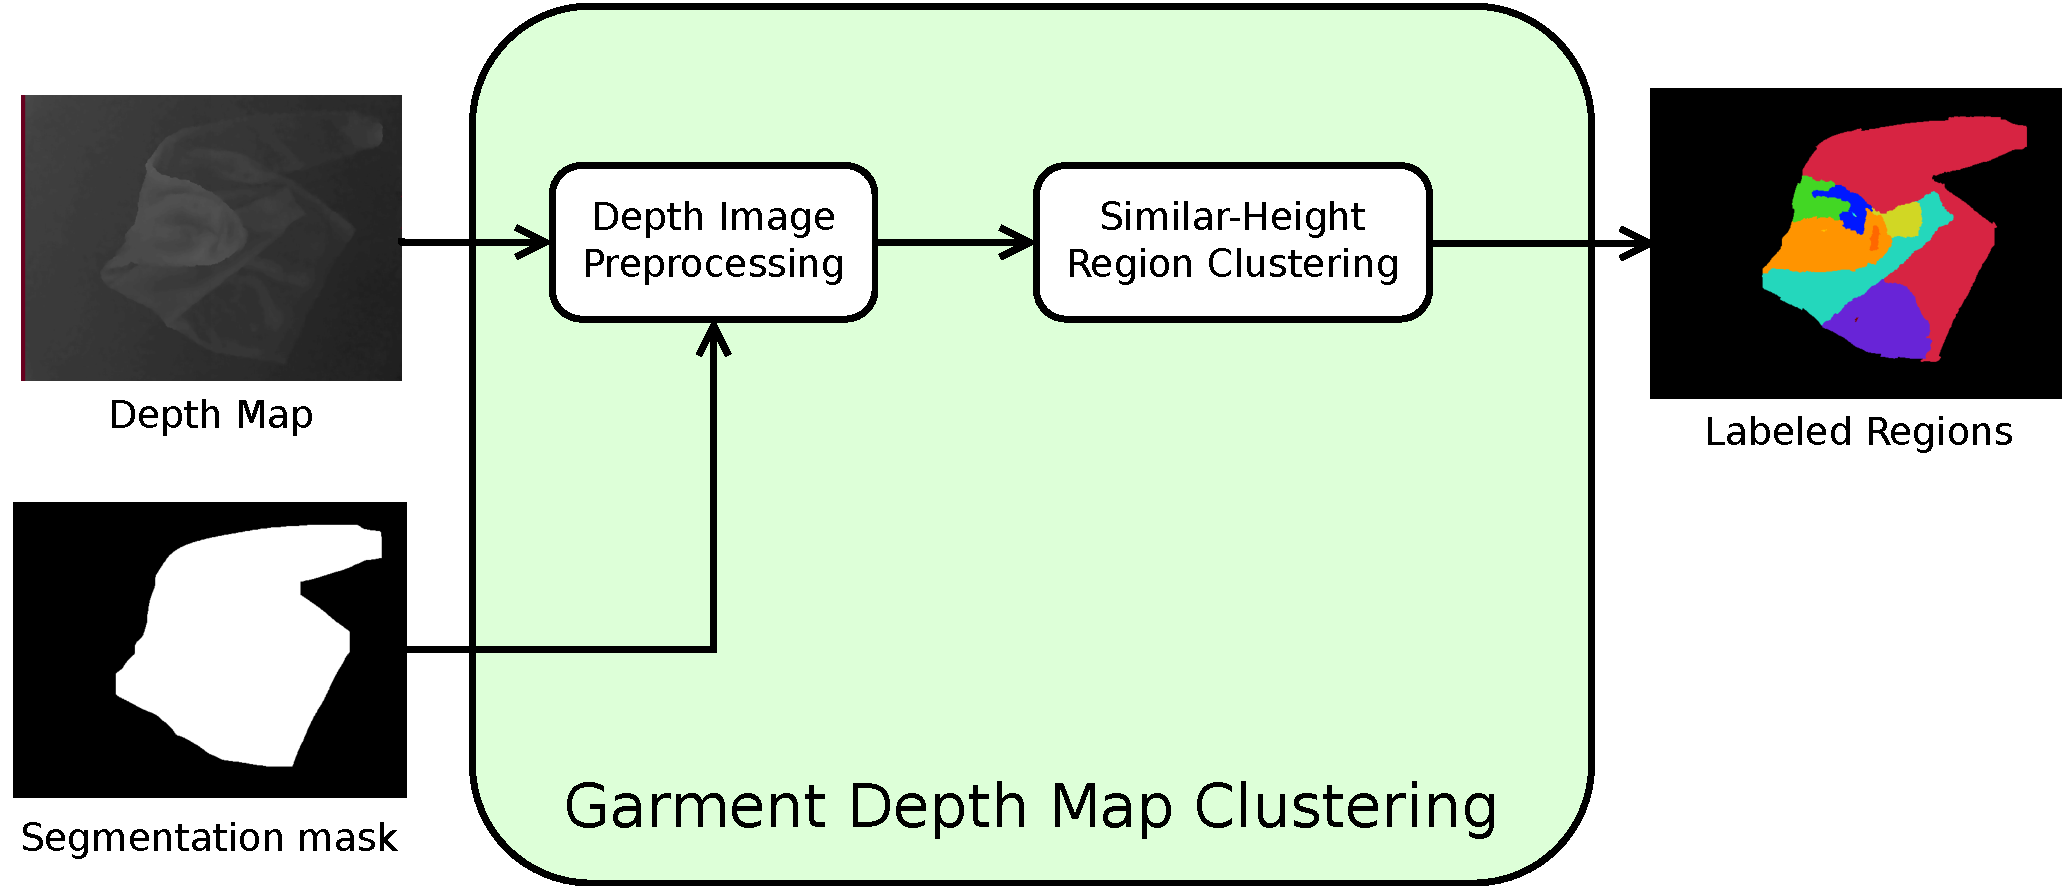
\includegraphics[width=\textwidth]
    {figures/Garment-depthmap-diagram.pdf}
    \caption[Block diagram showing an overview of the Garment Depth Map Clustering stage and its different steps.]
    {Block diagram showing an overview of the Garment Depth Map Clustering stage and its different steps. The inputs of this stage are the depth map image and the segmentation mask obtained in the previous stage. These inputs are combined and preprocessed in order to apply the clustering step. The output of this stage are the labels of the different cluster regions.}
    \label{fig:garment_clustering_blocks}
\end{figure}

In this stage, the depth image data is preprocessed using the segmentation results from the previous stage to remove all depth data not related to the garment. Then, it applies a Watershed transform algorithm to find the different similar-height regions, that will be analyzed in the last stage to select the most suitable manipulation points to unfold the garment. 

As mentioned before, some of these regions of similar height correspond to overlappìng regions of the garment, whose order can be determined using the average depth value of the pixels in each region. The garment region with the lowerst height value then corresponds to the region of the garment underneath those overlapping regions.

Once the different regions are labeled, those labeled clusters are passed to the next stage in order to determine the \comment{uppermost }fold and the most suitable unfolding direction.

\section{Depth Image Preprocessing}
\label{depth_image_preprocessing}

This step prepares the input depth data from the sensors to be used in later steps. The raw depth image data obtained from the robot sensors cannot be used directly, as it contains data related to outliers and noise. The data coming from the table on which the garment lies is also present in this image. Therefore, this data requires some treatment before it can be processed in the next step (section \ref{garment_clustering_watershed}). 

For that purpose, a required input of this step, the garment mask calculated in the previous stage, is applied to the depth image of the garment. The objective is to discard the information related to the table. After this process only information about the garment is present on the depth image.

The depth input data comes as a distance from the sensor to each pixel. As the next step will treat the depth data as a greyscale image, the remaining garment depth data needs to be normalized to the 8-bit range of a typical greyscale image. By normalizing the data we ensure that we are using the maximum resolution available (256 grey levels) to represent all the depth variability in the depth image. This helps the next step to find similar-height regions more accurately.

Figure \ref{fig:depth_map_preprocessing}  shows a comparison between the raw input depth data and the data after this processing step. \comment{Lorem ipsum dolor sit amet, consectetur adipiscing elit. Donec a diam lectus. Sed sit amet ipsum mauris. Maecenas congue ligula ac quam viverra nec consectetur ante hendrerit. Donec et mollis dolor.}

\begin{figure}[htbp]
	\centering
    \begin{subfigure}[l]{0.495\textwidth}
	    \centering
    	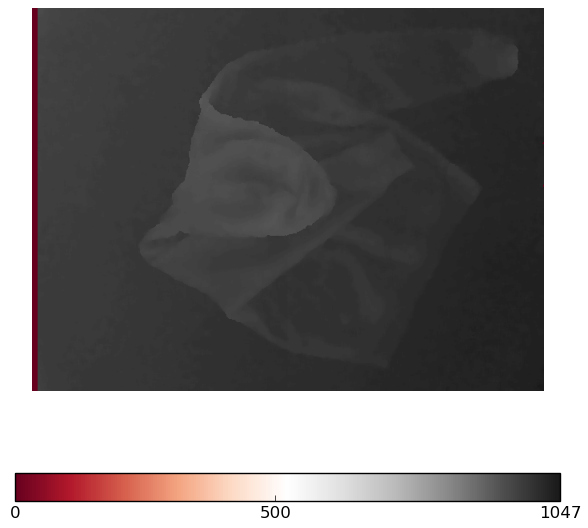
\includegraphics[width=\textwidth]
    	{figures/Depthmap-Raw-Depthmap-with-colorbar.png}
    	\caption{Before}
	\end{subfigure}
	~
    \begin{subfigure}[r]{0.485\textwidth}
	    \centering
    	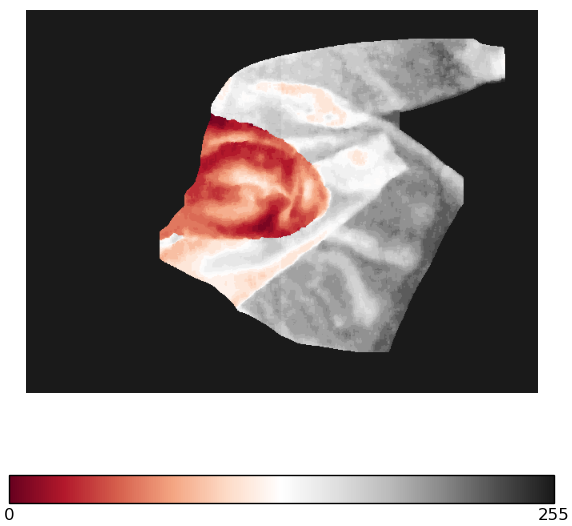
\includegraphics[width=\textwidth]
    	{figures/Depthmap-Normalized-Depthmap-with-colorbar.png}
    	\caption{After}
    	\end{subfigure} 
    \caption[Depth image before and after preprocessing.]
    {Depth image before and after preprocessing. \juansays{Note that (barras) indicate close are red, far are grey. //} \juansays{Mayoría imagen izquierda en grises, despues nota sobre franja roja}  On the left image, a red bar is shown in the leftmost part of the image, corresponding to some values captured by the sensor with errors. Points closer to the camera are shown lighter, whereas points futher from the camera are shown with darker gray levels. Units of the left image are mm. On the right image, representing the depth image after the preprocessing stage, it can be observed that the depth image now uses all the \comment{dynamic range}, coded as an 8-bit unsigned char.}
    \label{fig:depth_map_preprocessing}
\end{figure}


\section{Similar-Height Region Clustering}
\label{garment_clustering_watershed}

Once the garment depth data is separated from the table depth data and normalized in the previous step, similar-height regions must be identified and labeled.

Grouping points according to a common feature such as height is a clustering problem, and several clustering methods and alternatives were described in section \ref{architecture:depth_map_clustering}. Some of the superpixel segmentation algorithms were tested during the development of this work, but finally a Watershed \cite{digabel1978iterative} algorithm was selected to perform the clustering. This algorithm is faster than other superpixel approaches, \comment{[...]}

The Watershed transform is a segmentation algorithm that considers a greyscale image as a topological surface where high intensity pixels correspond to peaks and hills, and low intensity pixels are equivalent to valleys. The algorithm fills the surface pouring water at each isolated valley. As the water level rises, the water from different sources will start to merge. To prevent them from merging, the algorithm constructs barriers at the merging regions, and continues this process of adding water and building barriers until all the peaks have been flooded. The resulting barriers are the segmentation result, where each region enclosed correspond to a segmented item. Figure \ref{fig:watershed_example} shows an example of applying the Watershed algorithm to segment coins.

\begin{figure}[htbp]
	\centering
    \begin{subfigure}[l]{0.49\textwidth}
	    \centering
    	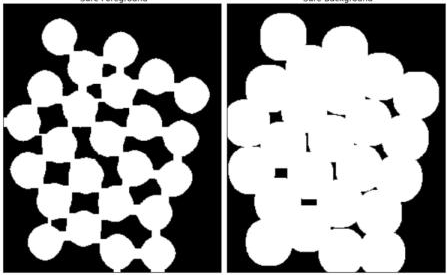
\includegraphics[width=\textwidth]
    	{figures/Watershed-example-02.png}
	\end{subfigure}
	~
    \begin{subfigure}[r]{0.49\textwidth}
	    \centering
    	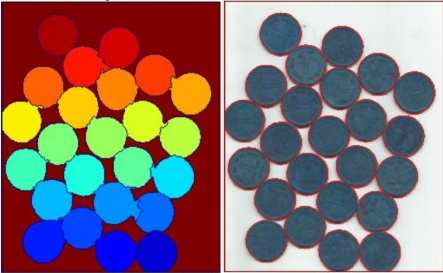
\includegraphics[width=\textwidth]
    	{figures/Watershed-example-03.png}
	\end{subfigure} 
    \caption[Several steps on segmenting coins with the Watershed Transform algorithm.]
    {Several steps on segmenting coins with the Watershed Transform algorithm\footnotemark. \juansays{Whaaaat?}The first and second images correspond to the erosion and dilatation of the thresholded coin image, representing sure foreground and sure background, respectively. Then, those images are combined and used as markers for Watershed segmentation. The result of this segmentation process is shown in the rightmost images, where each coin is labeled with a different color in the third image, and then marked with a circle in the fourth image. }
    \label{fig:watershed_example}
\end{figure}

\footnotetext{Source:\stdurl{http://docs.opencv.org/master/d3/db4/tutorial_py_watershed.html} , last accessed: \today}

A denoising process is performed before applying the Watershed transform, which is the actual clustering process. We use a Total Variation filter \cite{chambolle2004algorithm} to produce a smoother image while maintaining the edges sharp. The Total Variation filter works by minimizing the integral of the norm of the image gradient. As a result of this filter, piecewise-constant images (``cartoon-like'' images) are obtained.

The Watershed segmentation algorithm is then applied to the depth image of the garment to locate the different parts that are overlapping each other. These regions are related to folded parts, that rest on top of other parts of the garment. 

As, in practice, flooding using local minima as markers \juansays{(Revisar "markers")} leads to over-segmentation, an enhanced version\footnote{\stdurl{http://scikit-image.org/docs/dev/auto_examples/segmentation/plot_marked_watershed.html}} of this algorithm  allows the user to specify other criteria for selecting the seed points. The gradient of the greyscale depth-image is computed, and regions where the gradient has a low value are selected as these seed points. These regions correspond to homogeneous and continous regions, which are good candidates to be used as markers.


The different garment regions obtained with Watershed were labeled and used as input for the next step. Figure \ref{fig:watershed_labels} shows the result of this process.


\begin{figure}[htbp]
	\centering
    \begin{subfigure}[l]{0.49\textwidth}
	    \centering
    	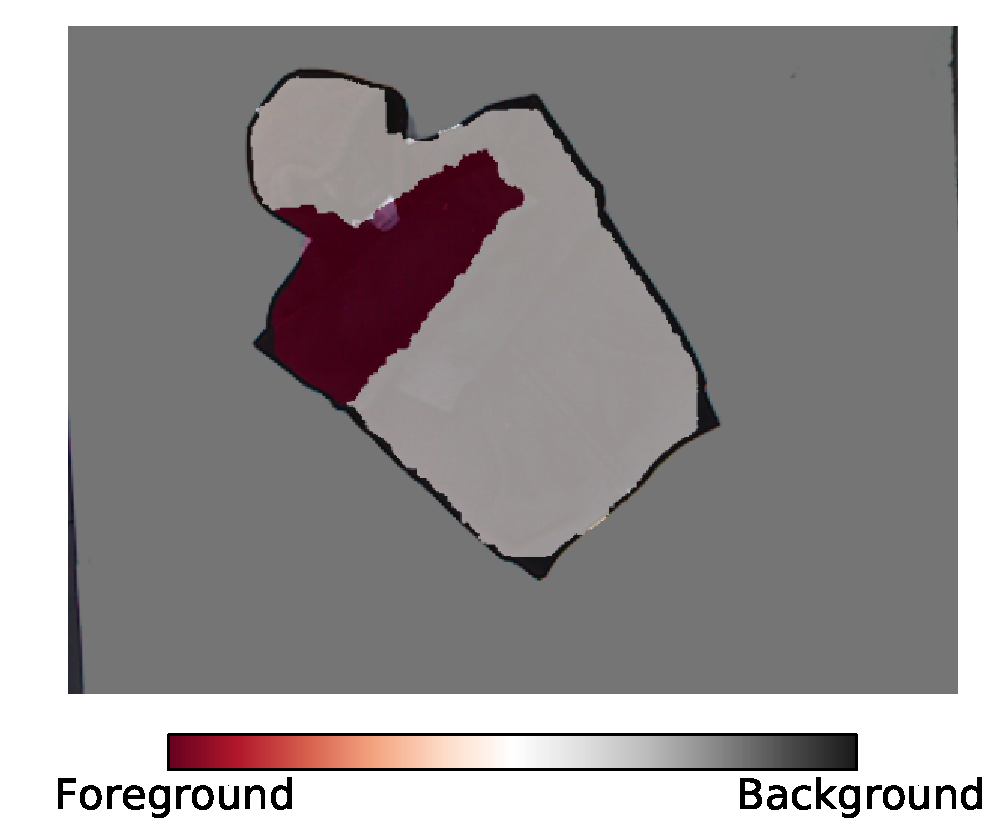
\includegraphics[width=\textwidth]
    	{figures/clustering/hoodie13-clustering.pdf}
	\end{subfigure}
	~
    \begin{subfigure}[r]{0.49\textwidth}
	    \centering
    	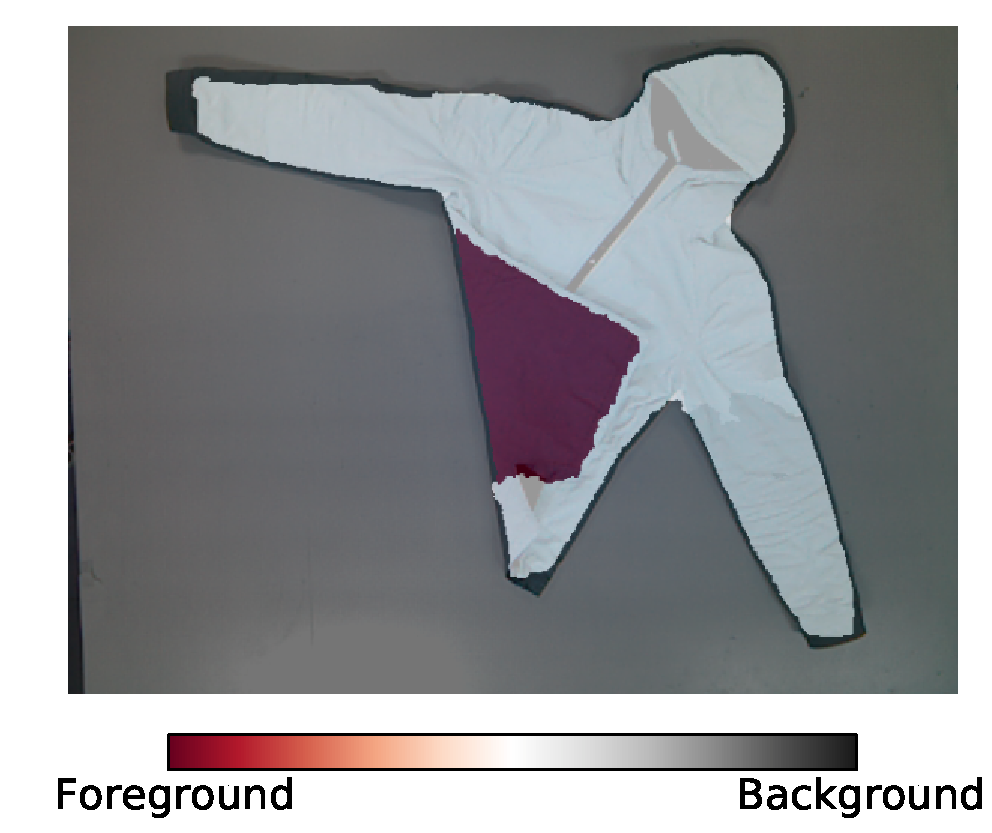
\includegraphics[width=\textwidth]
    	{figures/clustering/jacket7-clustering.pdf}
	\end{subfigure} 
	~
	\begin{subfigure}[l]{0.49\textwidth}
	    \centering
    	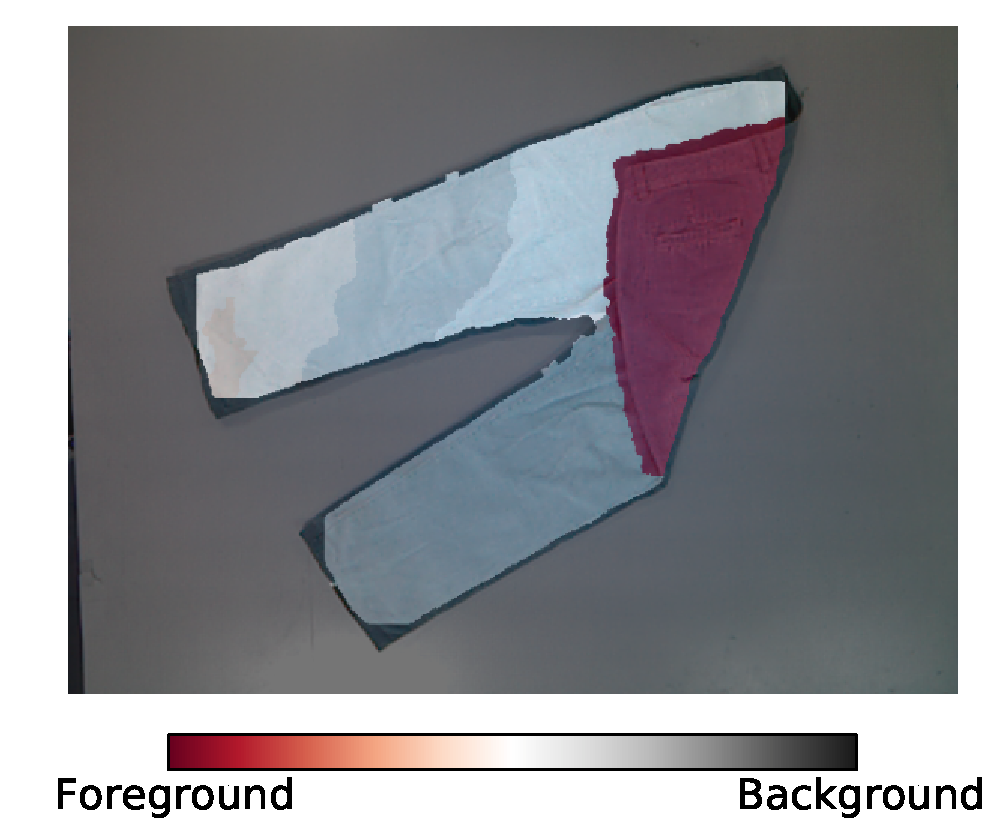
\includegraphics[width=\textwidth]
    	{figures/clustering/pants3-clustering.pdf}
	\end{subfigure}
	~
    \begin{subfigure}[r]{0.49\textwidth}
	    \centering
    	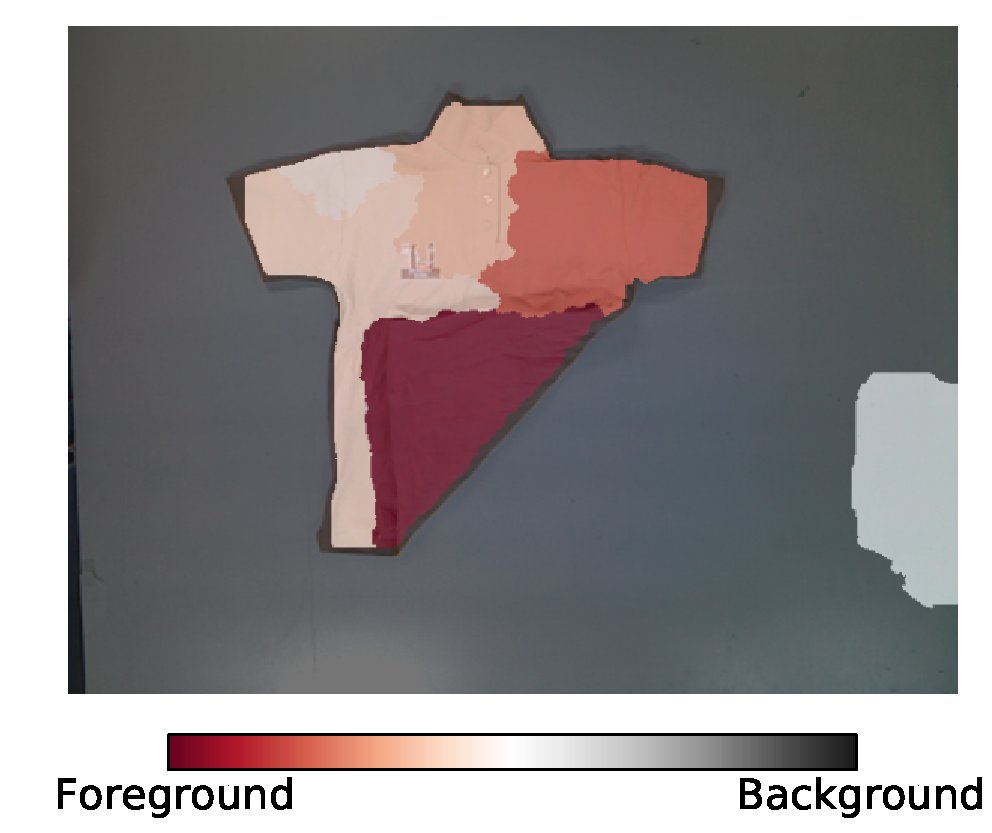
\includegraphics[width=\textwidth]
    	{figures/clustering/polo6-clustering.pdf}
	\end{subfigure}
	~
	\begin{subfigure}[l]{0.49\textwidth}
	    \centering
    	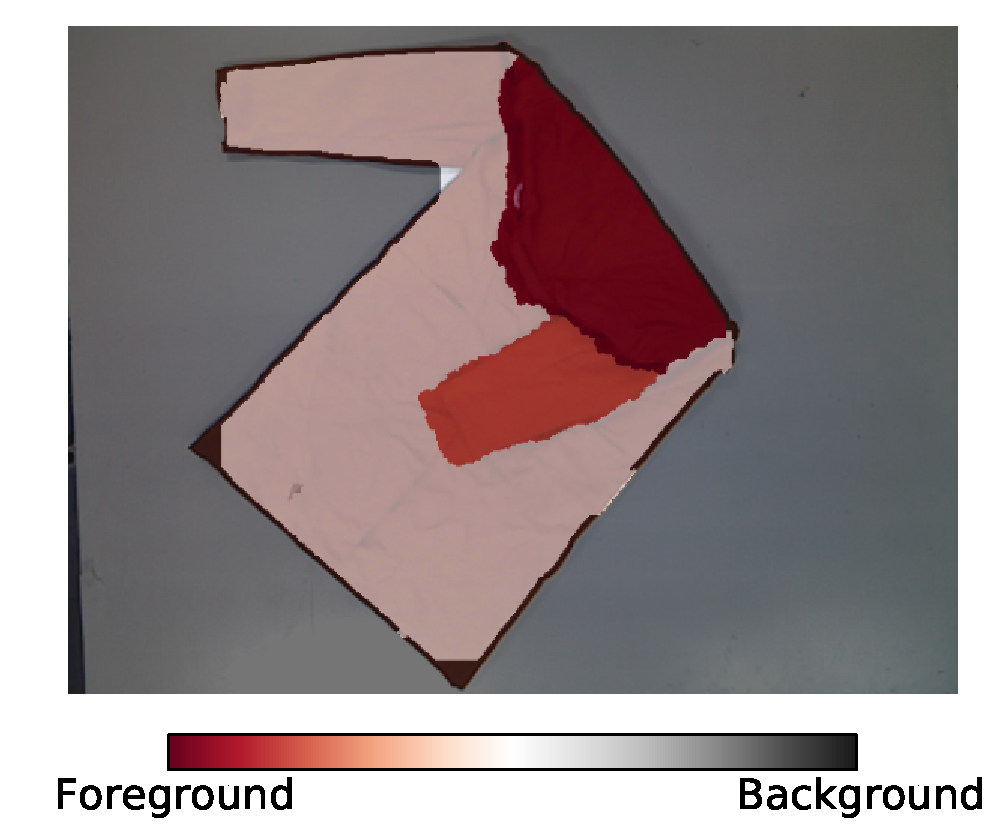
\includegraphics[width=\textwidth]
    	{figures/clustering/robe19-clustering.pdf}
	\end{subfigure}
	~
    \begin{subfigure}[r]{0.49\textwidth}
	    \centering
    	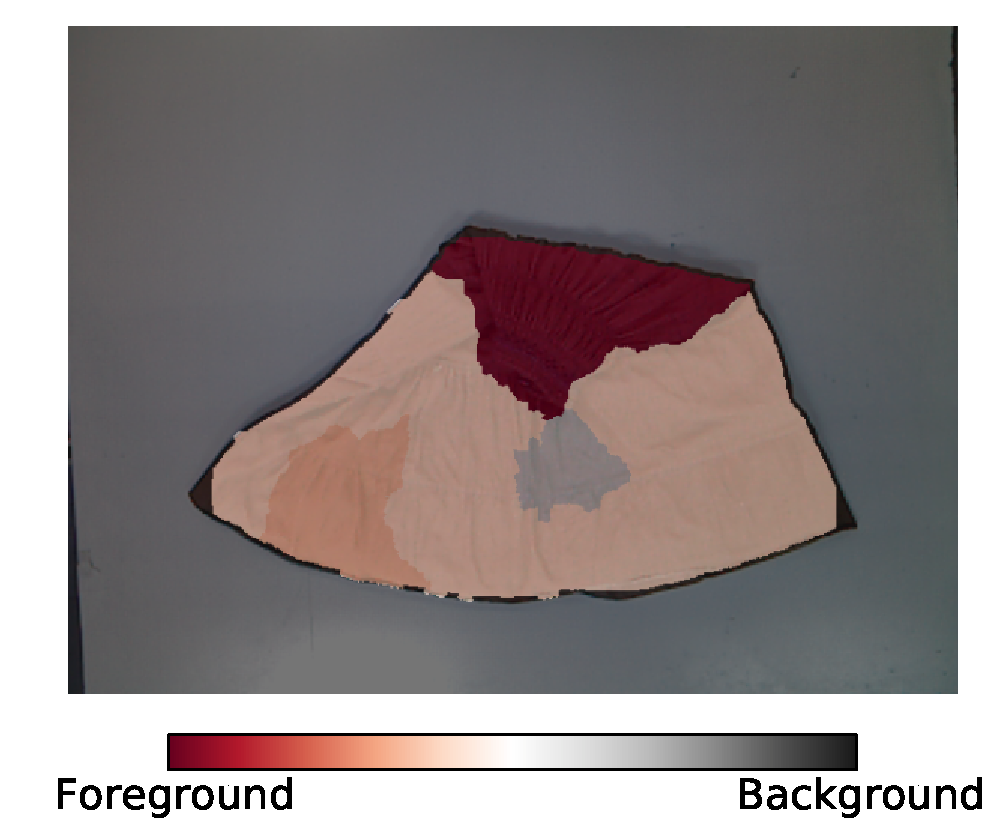
\includegraphics[width=\textwidth]
    	{figures/clustering/skirt17-clustering.pdf}
	\end{subfigure} 
    \caption[The normalized depth images for different clothes are shown on the left side.]
    {The normalized depth images for different clothes are shown on the left side. The grey level is related to the height of the point as detected by the RGB-D sensor. A darker grey level indicates the points are closer to the sensor. On the right side, the labeled image returned by watershed algorithm is presented, where each color represents a region of similar height.}
    \label{fig:watershed_labels}
\end{figure}

\comment{Lorem ipsum dolor sit amet, consectetur adipiscing elit. Donec a diam lectus. Sed sit amet ipsum mauris. Maecenas congue ligula ac quam viverra nec consectetur ante hendrerit. Donec et mollis dolor. Praesent et diam eget libero egestas mattis sit amet vitae augue. Nam tincidunt congue enim, ut porta lorem lacinia consectetur. Donec ut libero sed arcu vehicula ultricies a non tortor. Lorem ipsum dolor sit amet, consectetur adipiscing elit. Aenean ut gravida lorem. Ut turpis felis, pulvinar a semper sed, adipiscing id dolor. Pellentesque auctor nisi id magna consequat sagittis. Curabitur dapibus enim sit amet elit pharetra tincidunt feugiat nisl imperdiet. Ut convallis libero in urna ultrices accumsan. Donec sed odio eros. Donec viverra mi quis quam pulvinar at malesuada arcu rhoncus. Cum sociis natoque penatibus et magnis dis parturient montes, nascetur ridiculus mus. In rutrum accumsan ultricies. Mauris vitae nisi at sem facilisis semper ac in est.}